\documentclass[a4paper,10pt]{article}\large
\usepackage{iplouccfg}
\usepackage{zhfontcfg}

\setlength{\parindent}{2em} 
\linespread{1.5}\selectfont
\pagestyle{fancy}
\lhead{}
\chead{}
\title{Itti视觉注意模型}
\author{赵红苗}
\date{2013年7月23日}
\begin{document}
\maketitle

\begin{abstract} 

在人类视觉信息处理中,总是迅速选择少数几个显著对象进行优先处理,而忽略或舍弃其他的非显著对象,该过程称为视觉注意。而现在在处理复杂场景的图像时要浪费大量时间与计算能力,增加了图像分析的复杂性。因此将视觉注意机制进行建模并引入计算机图像处理的计算中有着重要的意义。通过深入研究视觉注意机制,Itti提出了视觉注意的计算模型。该模型构建了一种生物神经框架来解释人类视觉注意,它将视觉生理功能适当简化并用计算模型表示出来,从而得到了比较有效的视觉注意模型。因为该模型具有很好的生理依据,计算速度比较快,效果也比较理想,所以得到了广泛的关注和应用,在该领域具有里程碑的意义。本文主要介绍Itti提出的视觉注意模型,通过对模型的认识和了解,从而为下一步模型的改进与完善工作奠定了基础。


\begin{description}
\item[关键词:视觉注意,  图像处理,   Itti模型,  生理依据]
\end{description}
%1、介绍视觉注意概念 2、视觉注意机制建模对图像处理的意义 3、通过对视觉注意机制的深入研究,Itti提出了视觉注意机制的模型(引出Itti模型) 4、大体介绍该模型及该模型的优点 5、对本文进行简单介绍

\end{abstract}

\newpage
\tableofcontents 
\newpage
\section{引言}
\subsection{视觉注意机制}

近年来,随着信息科学技术的发展,图像数据的规模变得越来越大,面对如此庞大的图像数据,如何能够快速而准确地完成各种图像分析任务己经成为人们研究的热点。传统的图像分析方法将图像中所有区域都被赋予相同的处理优先等级,然而很多图像分析任务诸如目标识别、图像检索、场景分析等所关心的内容通常仅占图像中很小的一部分,因此,这种全面加工不但增加了分析过程的复杂性,而且带来了许多不必要的计算浪费。而对于人来说,当人睁开眼睛后,每一时刻都接受到大量的外界信息,处于被“信息轰炸”的状态中,生理学与心理学方面的研究表明人类处理信息的能力也是有限的,但我们依然没有被海量的视觉信息击垮。因为人类视觉系统在面对复杂场景时,不可能同时处理这么多的信息,会迅速将注意力集中在少数显著的区域,并利用自身的能力对其优先处理,这个过程称作视觉注意。


视觉注意起初是一个心理学概念,随着神经生物学的发展,人们开始定量的研究视觉注意机制,并且视觉注意的生理基础被逐渐了解。视觉注意也是一个多学科多交叉的研究领域,得到了心理学、认知神经科学、计算机科学等多学科的广泛关注,是近年来的研究热点之一。视觉注意机制的机理是生物视觉信息处理过程中一个非常重要、但又难以描述清楚的问题。按照对视觉信息的处理方式划分,可以将视觉注意过程分为两部分,分别为自底向上和自顶向下的视觉注意。自底向上的视觉注意由数据驱动、独立于具体任务,速度很快,一般产生于看到图像的20-50毫秒。而自顶向下的视觉注意受意识支配、依赖于具体任务,因此速度较慢,一般产生于看到图像的200毫秒以后。针对上述视觉注意的过程和特点,认知心理学的研究学者提出了许多假设,较具代表性的有\cite{4:article}Treisman和Gelade的特征融合理论、Treisman的聚光灯假设、Schneider和Shiffrin的二元理论、Broatbent的过滤器模型和的能量分配模型等。在上述的众多理论和模型中,Treisman的特征融合理论和Koch的神经生物学框架\cite{5:article}奠定了视觉注意建模在计算机中的可计算性基础。这两个理论基础将在后文展开。


将视觉注意机制引入到图像处理领域是非常必要且有意义的,它可以提供观察者可能感兴趣的对象区域信息,帮助制定合理的计算资源分配方案,从而可以大幅地提升已有图像处理系统的运行效率。将传统的图像处理过程和人类的视觉注意相结合,提取和图像分析任务有关的内容并优先处理,形成一套合理的资源分配方案来引导图像处理,使计算机具有类似人类选择性和主动性的信息处理能力,这是本领域的主要研究目的。

%1、提出的背景(为什么要引入视觉注意)2、详细介绍视觉注意(其中不要忘了视觉注意的两个过程B-u、T-D)3、引入视觉注意的意义

\subsection{Itti计算模型}

\subsubsection{Itti模型的理论基础}

\begin{itemize}
\item 特征融合理论
\end{itemize} 

Treisman和Gelade在年提出了特征融合理论。它是目前视觉注意机制建模领域最具影响力的一个理论基础。特征融合理论把感知对象分解为特征和实体两部分,认为特征是一系列的属性值,实体则是特征的组合。这些特征是依附实体而存在的,在开始的时候未被解析,全部特征以结合在一起的状态存在。随后便分为空间特征与非空间特征,分别沿人脑的和两条通路并行地达到不同的部位。这时,空间特征和非空间特征仍具有联系,它们所在的部位在主客观的因素作用下,有的被抑制,有的则被激活。处于高激活状态部位的特征被选择而得到注意,而这些特征再次融合形成实体的综合特征,并通过语义表的匹配得到了识别。对于那些处于低激活状态的特征不能相互融合,其实体也不能得到注意。

特征融合理论将视觉加工分为两个阶段,预注意阶段和特征融合阶段。预注意阶段的特征加工是高速并行的,而注意期的对象加工是低速串行的。注意焦点是联系这二者的枢纽,它从特征加工中获得特征的选择依据,并为后面的对象加工提供引导。下面将分别予以介绍:


(1)预注意阶段

预注意阶段又称注意前期,它的加工帮助人们快速地从周围的环境中进行目的性搜索。人类视觉系统从光的刺激中快速抽取模式信息,是一种平行的自动处理过程。在这个阶段,视觉系统只能抽取彼此独立的特征,诸如颜色、方向、尺寸、亮度、纹理和运动等特征。这些特征彼此相对独立,并且不受实体约束,在位置上是不受主观影响的。这个阶段所提取的特征被称为早期视觉特征或初级视觉特征。视觉系统对于各个特征独立并行地处理,在每个特征通道中形成一幅特征图。整个过程处理速度较快,
并且彼此不相互影响。

(2)特征融合阶段

特征融合阶段又称注意期,在这个阶段感知系统把彼此独立分离的特征统一地联系起来,形成对某一对象的综合表征。这个阶段需要对特征进行位置确定,这种对特征进行心理定位的表征称为位置地图。这个阶段由于处理特征的位置信息,需要集中注意来把原始的、彼此分离的特征融合形成一个实体,因而通常这个过程处理的速度相对较慢。


\begin{itemize}
\item Koch神经生物学框架
\end{itemize} 


许多心理学的研究工作表明,在视域中对于对象的检测、定位和识别极可能是一个两阶段的人类视觉感知过程。第一个阶段被称为“预注意阶段”,在这个阶段,简单的早期特征在整个视域中被并行且快速的处理。在第二个阶段,称为“注意阶段”,一个特定的处理焦点,通常称为“注意焦点”,它被导引到视域中的某些特定的位置。对于复杂的形式分析和对象的识别只与第二个阶段相关。那么在的神经生物学模型中,分别用显著度图和选择性映射来描述上述两个阶段。

(1)显著度图

对于不同的特征通道,可以认为在一个视觉场景中某个位置的显著程度决定了不同特征图中相对应单元的主动性。它们的主动性越高,在视域中对应位置的显著度也就越高。这样,不同的特征通道在一个特定的特征空间里面协同形成一种显著性。那么为了可以直接访问视域中每个位置的显著性,我们假设存在一幅“显著度图”。这幅显著度图融合了每个独立的特征通道的信息,形成了一种全局的显著度。与原始特征图中某个位置相对应的那些点则映射到显著度图中的一个单元。这种关联并不是不相关的,只要增强特征图中的显著性就会增加在显著度图中的显著度。那么这幅图像就给出了对于视觉环境的一种“偏见”,着重强调了视域中的感兴趣区域或显著区域。由于显著度图仍然是早期视觉系统的一部分,它更倾向于通过简单的视觉特征来描述显著对象的显著性,诸如颜色、运动、深度和方向特征。那么一个位置的显著度主要取决于该位置在颜色、运动、深度和方向等特征上与周围的区域的差异程度。尽管这样,也很可能对于不同对象不同特征贡献的相对权重会发生变化。综上所述,第一阶段,也就是显著度图的形成阶段。

在视觉注意的第一阶段预注意阶段,人眼是通过在不同的特征通道快速且并行地抽取早期的视觉特征,并将这些特征予以融合来形成一幅潜在的视觉显著度图。这幅视觉显著度图描述了图像中的每个位置的视觉显著程度,对于图像中的感兴趣区域和显著区域具有一定的倾向性。这样便于后一阶段对象的定位与识别。


(2)选择性映射

接下来,我们需要构建一种机制来确保在这个阶段只有那些与最显著的位置相关的属性被映射到后续的处理中。换句话说,我们需要给出一种机制来让那些“注意点”或“选择点”相关的属性可以被提交到后面的处理中。在这里等人认为早期视觉特征的选择是优于选择性映射的,并认为在选择性映射这个阶段各个特征的融合己经完成,因此采用Winner-Taken-All网络法则来构建显著度图各个位置区域之间的竞争关系,并以此作为后面的视点转移过程的基础。

对于一个多输入的网络,假设对于每个输入$x_{i}$,都对应一个相应的输出$y_{i}$,那么网络法则要求:
\begin{equation}
y_{i}=0\qquad x_{i} < \textrm{max} x_{i}
\end{equation}
\begin{equation}
y_{i}=f(x_{i})\qquad x_{i} = \textrm{max} x_{i}
\end{equation}
从上面两式可以看出只有最大的输入可以获得输入,其他的输入都被屏蔽了。这样也就符合是视觉注意机制中的单焦点性。为了防止注意焦点一直停留在显著度图中最为显著的位置,等人还设计了相应的抑制返回机制。对于己经注意过的位置区域,将其显著度值设置为最小,保证该位置在后续竞争中则不会再次出现。对于视点转移过程的模拟,等人认为视点转移遵从以下两点原则:1、近邻优先。视觉注意机制总是倾向于选择距离当前注意焦点近的显著区域作为下一个注意焦点。2、相似优先。视觉注意机制总是倾向于选择内容属性上如颜色、方向、运动等特征与当前注意焦点相似的显著区域作为下一个注意焦点。


综上所述,Koch等人的神经生物学框架给出了一套较为完整的视觉注意机制建模的整体思路和框架,其中的贡献有视觉注意的两阶段性、显著度图、以及抑制返回机制和视点转移的相关原则。这使得神经生物学框架备受关注,奠定了视觉注意机制建模领域重要的理论基础。1998年Koch的学生成功地构建出了首个基于该框架的计算模型。

%因为这两个是Itti模型提出的理论基础,所以想在这里介绍一下

\subsubsection{Itti计算模型}

对于Itti提出的视觉注意模型\cite{1:article},大体思想是在空间域中计算图像中各个位置的视觉显著程度,即采用显著度来衡量。首先定义图像中的感知单元,通常可以是像素或者图像块。计算每个感知单元相对于四周邻域或者整幅图像在不同特征下的相对对比度,将这种对比度作为该位置的显著度来衡量,并定义特征之间的竞争或者融合的关系,最终确定图像中每个位置的显著度,形成一幅视觉显著度图。再根据显著度图的特点,定义某种机制来选择图像中的显著区域,进而实现视觉注意机制的模拟。其模型如图\ref{fig:1}所示:

\begin{figure}[!htb]
\centering
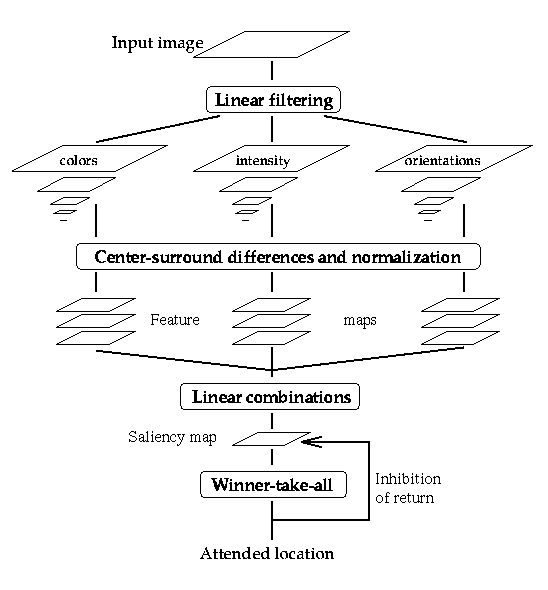
\includegraphics[width=0.5\textwidth]{IttiModel.png}
\caption{Itti视觉注意模型}\label{fig:1} 
\end{figure}


该模型大致分为以下五个部分:

1. 模拟视网膜与初级视皮层从输入图像中提取多种底层视觉特征,如颜色、方向、亮度等等


2. 模拟中央-周围拮抗感受野计算各个特征内的显著图


3. 模拟侧抑制机制计算特征显著图的竞争


4. 模拟特征融合机制进行特征显著图的融合


5. 模拟视皮层中的反馈连接实现注意点的转移


%1、总体介绍Itti提出的模型(附图Itti视觉注意模型)
%2、该模型的组成部分
\subsection{本文结构安排}
本文主要对Itti提出的视觉注意模型进行研究,对Itti模型\cite{2:article}的每个环节进行详细阐述,包括特征、特征显著图、竞争、融合等步骤。通过本文的介绍,从而更深刻的理解Itti的建模机制。


\section{前期视觉特征提取}

特征提取是视觉注意建模过程中的关键步骤,它将视觉感受到的刺激通过特征通道反映到形成的图像中。同时,它也是图像内容转化为定量可计算信息描述的关键。

在人类视觉系统中,视网膜的感光细胞有两种,视杆细胞能够感知亮度信息,而视锥细胞能够感知颜色信息。在初级视觉皮层中,存在着方位柱、颜色柱等生理结构将视觉信息进一步细分处理。基于这样的生理基础,Itti 选择提取图像的亮度、颜色和方向特征来模拟这些生理功能。


\subsection{亮度特征提取}

亮度信息是最基本的视觉信息,它直接由视网膜的视杆细胞产生,是最基本的视觉信息,视觉系统中的其他信息很多也是由亮度而来。而从计算的角度考虑,亮度特征也足够用于多数图像处理任务,比如分割、识别,同时计算量远小于彩色特征。一些特殊成像方法得到的图像没有颜色信息,直接利用获取的亮度信息。


设$r$,$g$,$b$为输入图像的红色、绿色、蓝色通道,则Itti原始模型中亮度特征可以简单的计算出来:

\begin{equation}
I=\frac{r+g+b}{3}
\end{equation}
后来对于Itti原始模型的扩展模型中,有一些参考了$RGB$颜色空间转$YIQ$颜色空间的公式,使用加权的平均公式,更加符合人眼感受:
\begin{equation}
I=0.299r+0.587g+0.144b
\end{equation}

\begin{figure}[!htb]
\centering
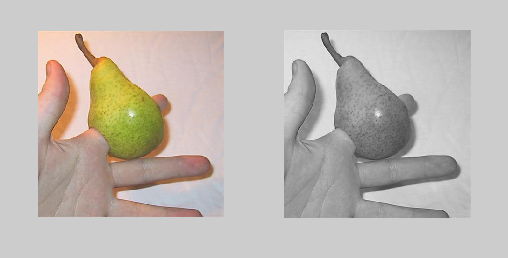
\includegraphics[width=0.7\textwidth]{Intensity.png}
\caption{亮度特征图}\label{fig:2} 
\end{figure}

\subsection{颜色特征提取}

颜色信息由视网膜的三种视锥细胞分别产生,而在初级视觉皮层中的颜色柱进行重新组合。颜色柱中的神经细胞对颜色的选择呈现双拮抗性质,即一种颜色使得细胞产生
兴奋,而另一种颜色使得能够抑制该细胞的兴奋。在人类视觉皮层中存在四种拮抗颜色对,分别是红-绿、绿-红、蓝-黄、黄-蓝。


首先为了去除颜色与亮度之间的耦合关系,用之前计算的亮度值 对 进行规一化处理。又因为视锥细胞只能在明亮的光线下感受颜色,所以只对亮度大于图像中最大亮度10\%的区域进行规一化,而其他区域的 均置为$0$。



数字图像一般只有红、绿、蓝三个颜色通道,为了得到黄色通道,Itti根据归一化后的 ,使用下面的公式计算广义上的红、绿、蓝、黄四个通道:

\begin{equation}
R=r-\frac{g+b}{2}
\end{equation}
\begin{equation}
G=r-\frac{r+b}{2}
\end{equation}
\begin{equation}
B=r-\frac{r+g}{2}
\end{equation}
\begin{equation}
Y=r+g-2(|r-g|+b)
\end{equation}
接下来利用这四个通道计算红-绿、蓝-黄颜色对。Itti模型巧妙地利用绝对值,表示了两个相反的颜色对中兴奋的那一种。因此红-绿与绿-红颜色对可以用一个公式表示:
\begin{equation}
RG=|R-G|
\end{equation}
\begin{equation}
BY=|B-Y|
\end{equation}
于是得到颜色特征图\ref{fig:3}。
\begin{figure}[!htb]
\centering
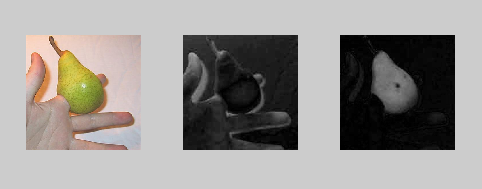
\includegraphics[width=0.8\textwidth]{Color.png}
\caption{颜色特征图}\label{fig:3} 
\end{figure}

\subsection{方向特征提取}

初级视觉皮层细胞对特定方向的刺激有强烈反应。Dennis Gabor经过研究发现,二维Gabor滤波器非常适合表示这种反应。二维Gabor滤波器是一种用于检测边缘的线性滤波器,由高斯核函数与一个余弦函数调制得到:
\begin{equation}
g(x,y;\lambda,\theta,\psi,\delta,\gamma)=exp\Big(-\frac{x'^2+\gamma^2y'^2}{2\delta^2}\Big)sin\big(\frac{2\pi x'}{\lambda}+\psi\big)
\end{equation}


其中$x'=xcos\theta+ysin\theta$,$y'=-xsin\theta+ycos\theta$。公式中$\lambda$表示余弦函数的波长,$\theta$表示Gabor滤波器的方向,$\psi$表示相位,$\gamma$表示空间长宽比,$\delta$表示高斯包络的标准差。


由于初级视觉皮层中有几千万个细胞,无法用模型将它们全部表示出来,Itti对这种生理结构进行了适当的简化。通过比较生理实验结果与模型的结果,固定次要变量,
设置$\lambda=7$,$\psi=0$,$\gamma=1$,$\delta=2.333$。而主要的变量是$\theta$,对应着Gabor滤波器的方向,Itti将连续的方向离散化,选择了4个最有代表性的方向:$0^\circ$,$45^\circ$,$90^\circ$,$135^\circ$,这样就构造出4个Gabor滤波器,分别对输入图像滤波,得到4个方向特征图,记作$O(\theta)$,其中$\theta=0^\circ,45^\circ,90^\circ,135^\circ$。其特征图如图\ref{fig:4}:
\begin{figure}[!htb]
\centering
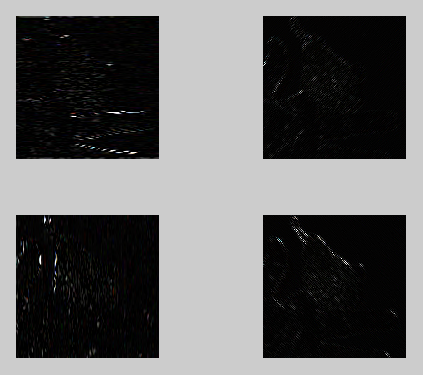
\includegraphics[width=0.8\textwidth]{Orientation.png}
\caption{方向特征图}\label{fig:4} 
\end{figure}

%包括基本的三种特征:I、C、O (附上特征提取前后的图片)
\section{特征显著图}

由于亮度、颜色、方向等等信息在外侧膝状体以及初级视觉皮层里都是并行处理的,而外侧膝状体与初级视觉皮层的细胞感受野基本都是同心圆的中央-周围拮抗感受野,
通过这种结构的感受野去除冗余信息,突出与周围反差较大的区域。因此这一步主要是对视觉系统中的同心圆拮抗感受野的模拟,分别对亮度、颜色、方向等特征图进行处理,得到各个特征的显著图。


1965年,Rodieck提出了同心圆拮抗感受野的数学模型\cite{6:article},它由两个高斯函数的差来表示:

\begin{equation}
DOG(r)=A\cdot exp\Big(-\frac{r^2}{\delta_{A}^{2}}\Big)+B\cdot exp\Big(-\frac{r^2}{\delta_{B}^{2}}\Big)
\end{equation}


其中$r$ 为感受野中的点到中心点的距离。当$A>B$且$\delta_{A}<\delta_{B}$时,式子对应On型感受野;当$A<B$且$\delta_{A}>\delta_{B}$时,式子对应 Off 型感受野。
\begin{figure}[!htb]
\centering
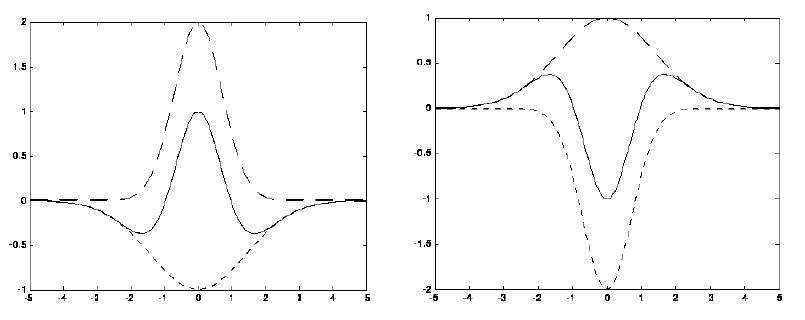
\includegraphics[width=0.9\textwidth]{DOG函数.png}
\caption{DOG函数}\label{fig:5} 
\end{figure}

Itti简化了这个模型,将这个模型看作一个线性滤波器,则滤波的结果等价于两个高斯滤波器滤波结果的差。因此Itti先用若干个不同方差的高斯滤波器对特征图像滤波,然后对这些滤波结果求差。最后对差求绝对值,以此来同时模拟On型感受野与Off型感受野中产生兴奋的那一种。


具体的说,Itti首先构造特征图像的高斯金字塔。高斯金字塔是一系列图像,每一层都是由前一层图像高斯滤波然后下采样得到。Itti构造的高斯金字塔中,共有9种尺度,每一种尺度的图像尺寸都是前一种的$1/2$。原始特征图像作为尺度0,则尺度1是对尺度0的图像进行高斯滤波,然后x与y方向均下采样至$1/2$大小。最后一个尺度是尺度8,对尺度7的图像高斯滤波并下采样,其x与y的尺寸是原始图像的$1/256$,其模型如图\ref{fig:6}所示

%\begin{figure}[!h]
%\begin{minipage}[t]{0.5\textwidth}
%\centering\includegraphics[width=2.5in]{1_11_s_GT.png}
%\caption{GT}
%\end{minipage} 
%\begin{minipage}[t]{0.5\textwidth}
%\includegraphics[width=2.5in]{1_11_s.png}
%\caption{Processed image}
%\end{minipage}
%\end{figure} 






\begin{figure}[!ht]
\begin{minipage}[c]{0.1\textwidth}
\centering
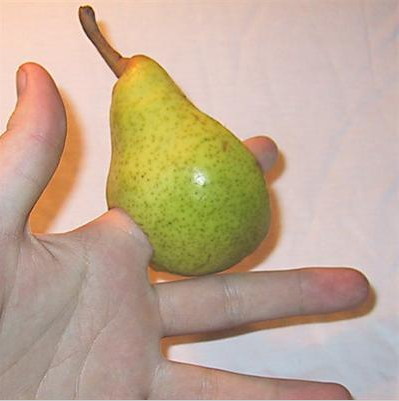
\includegraphics[width=1.25in]{figures/pyramidal_0.png}
\end{minipage} 
\hspace{12ex}
\begin{minipage}[c]{0.1\textwidth}
\centering
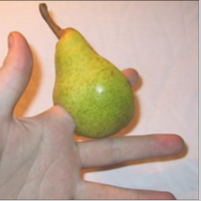
\includegraphics[width=0.625in]{figures/pyramidal_1.png}
\end{minipage}
\hspace{1ex}
\begin{minipage}[c]{0.1\textwidth}
\centering
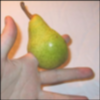
\includegraphics[width=0.3125in]{figures/pyramidal_2.png}
\end{minipage}
%\hspace{1ex}
\begin{minipage}[c]{0.1\textwidth}
\centering
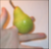
\includegraphics[width=0.15625in]{figures/pyramidal_3.png}
\end{minipage}
\begin{minipage}[c]{0.1\textwidth}
\centering
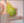
\includegraphics[width=0.078125in]{figures/pyramidal_4.png}
\end{minipage}
%\hspace{1ex}
\begin{minipage}[c]{0.1\textwidth}
\centering
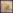
\includegraphics[width=0.0390625in]{figures/pyramidal_5.png}
\end{minipage}
%\hspace{1ex}
\begin{minipage}[c]{0.1\textwidth}
\centering
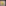
\includegraphics[width=0.01953125in]{figures/pyramidal_6.png}
\end{minipage}
%\hspace{1ex}
\begin{minipage}[c]{0.1\textwidth}
\centering

\includegraphics[width=0.009765625in]{figures/pyramidal_7.png}
\end{minipage}
\caption{高斯金字塔}\label{fig:6}
\end{figure} 


这样9个不同尺度的图像,等价于对原始图像使用不同方差的高斯滤波器滤波的结果。因此将这些图像相减就可以模拟同心圆感受野。Itti选择尺度2到尺度4的图像减去相差3、4个尺度的另一个图像,即一副图像的尺度是$c$,则另一幅图像的尺度是$c+s$,其中$c=2,3,4$,$s=3,4$。任取一组c与s的值,都能确定两幅图像。先将尺寸较小的那幅图像放大,使得两幅图像尺寸相同,然后将这两幅图像相减,将这种减法记作$\ominus$。再求绝对值,就得到了一个同心圆感受野的模拟结果。总共能得到6个不同形状的同心圆感受野的结果,通过共用高斯金字塔的尺度,减少了计算量,同时能够避免边缘效应。

\begin{figure}[!htb]
\centering
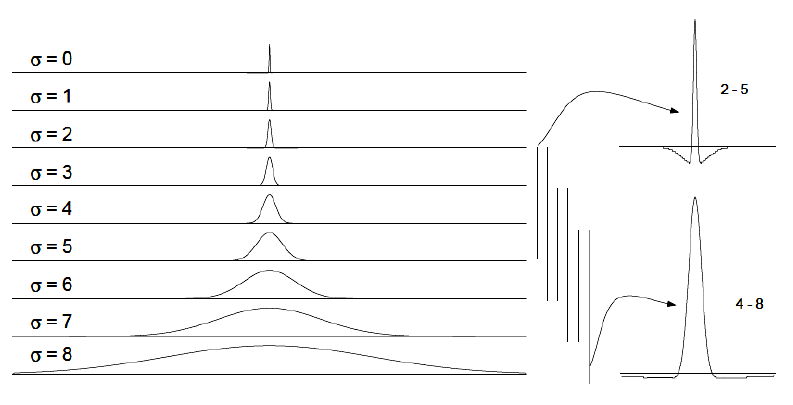
\includegraphics[width=0.9\textwidth]{DOG滤波.png}
\caption{利用高斯金字塔实现DOG滤波}
\label{fig:7} 
\end{figure}

这种处理对各个特征分别进行。对于亮度特征图$I$,首先构造高斯金字塔$I(\delta)$,其中$\delta=0,1,2\ldots,8$。然后计算亮度显著图$I(c,s)=|I(c)\ominus I(c+s)|$,其中$c=2,3,4$,$s=3,4$。如图\ref{fig:8}所示。同样的对于两个颜色特征图RG与BY,构造高斯金字塔$RG(c,s)$与$BY(c,s)$,然后计算颜色显著图$RG(c,s)=|RG(c)\ominus RG(c+s)|$,$BY(c,s)=|BY(c)\ominus BY(c+s)|$。对于方向特征$O(\theta)$,其中$\theta=0^\circ,45^\circ,90^\circ,135^\circ$,构造高斯金字塔$O(\theta,\delta)$,然后计算方向显著图$O(\theta,c,s)=|O(\theta,c)\ominus O(\theta,c+s)|$。这样对于 7 个特征图像,一共计算了42个特征显著图。
\begin{figure}[!ht]
\begin{minipage}[c]{0.31\textwidth}
\centering
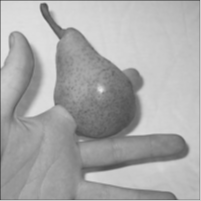
\includegraphics[width=1.25in]{image1.png}
\end{minipage}
\hspace{1ex}
\begin{minipage}[c]{0.31\textwidth}
\centering
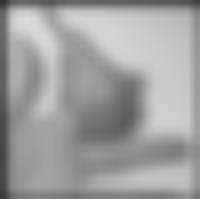
\includegraphics[width=1.25in]{image1_4.png}
\end{minipage}
\hspace{1ex}
\begin{minipage}[c]{0.31\textwidth}
\centering
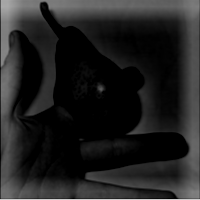
\includegraphics[width=1.25in]{feature1_4.png}
\end{minipage}
\caption{一个特征显著图的形成}\label{fig:8}
\end{figure} 

%1、构造特征金字塔(附金字塔构造原理图)2、利用中央周围算子获取42幅特征显著图

\section{特征显著图竞争}

特征显著图的竞争是为了模拟神经元的侧抑制机制。邻近的神经元之间能够彼此抑制对方的兴奋,从而去除相似的冗余信息,并增强反差信息。

\subsection{不做竞争的处理}

最朴素的方法就是不作任何竞争的处理,仅仅考虑到不同特征显著图的计算方法与参数的不同,导致特征显著图的取值范围各不相同,因此对各个特征显著图进行归一化处理。但这样做的问题也非常明显,比如在一幅图中,亮度、颜色均相同的条纹,只有方向不同,因此从亮度显著图以及颜色显著图均无法区分出真正显著的区域,而倾斜的方向显著图甚至将真正显著的区域排除在外,只有倾斜的方向显著图突出了真正的显著区域。所以亮度、颜色以及其他方向显著图都是无效的信息。


心理实验表明真正引起视觉注意的往往是图像中占少数的区域,所以如果某个特征显著图中的显著区域过多,很可能是不应该显著的背景。模拟侧抑制机制,让特征图内部产生竞争,使得大量出现的显著区域相互抑制,少量出现的显著区域得到突出,可以很好地解决这个问题。

\subsection{基于内容的全局缩放方法}

Itti在最初的论文中提出了这种基于内容的全局缩放方法来模拟侧抑制机制。这种竞争可以定义为归一化算子$N(\cdot)$,其具体计算过程计算如下:


(1)对于每幅特征图,将图中的显著度值归一到固定区间$[0,\ldots,M]$,这样做是为了消除因不同特征通道中显著度值分布的区间不同而产生的放大效应。


(2)寻找图中的全局最大值$M$,计算所有其他局部最大值的平均值$\bar{m}$。仅仅考虑极大值可以忽略图像中的均匀区域,从而仅比较有意义的区域。


(3)将显著图中的每个位置均乘以放大系数$(M-\bar{m})^2$,全局极大值与平均极大值的差反映了特征显著图中显著区域的分布情况。如果显著区域很多,则局部极大值的均值就接近于全局极大值,$(M-\bar{m})^2$就非常小,与特征显著图相乘之后使得特征显著图被整体抑制。反之,如果显著区域很少,除了全局极大值以外的局部极大值都比较小,$(M-\bar{m})^2$就比较大,与特征显著图相乘之后使得特征显著图增强。


其缩放方法如图\ref{fig:9}所示:






\begin{comment}
首先要对特征图进行归一化处理。对于每个特征显著图,找出它的全局极大值$M$,并计算除了$M$以外的局部极大值的均值 。仅仅考虑极大值可以忽略图像中的均匀区域,从而仅比较有意义的区域。最后将该特征显著图乘以$(M-\bar{m})^2$。全局极大值与平均极大值的差反映了特征显著图中显著区域的分布情况。如果显著区域很多,则局部极大值的均值就接近于全局极大值,$(M-\bar{m})^2$就非常小,与特征显著图相乘之后使得特征显著图被整体抑制。反之,如果显著区域很少,除了全局极大值以外的局部极大值都比较小,$(M-\bar{m})^2$就比较大,与特征显著图相乘之后使得特征显著图增强。其缩放方法如图\ref{fig:9}所示:
\end{comment}


\begin{figure}[!htb]
\centering
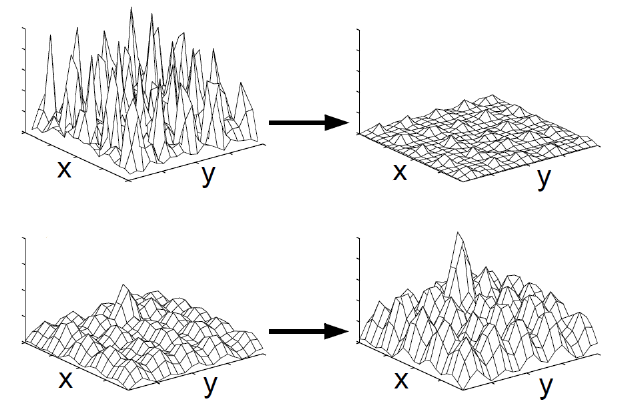
\includegraphics[width=0.7\textwidth]{全局缩放.png}
\caption{基于内容的全局缩放方法}
\label{fig:9} 
\end{figure}

上述的归一化算子$N(\cdot)$将每幅特征图中的潜在的显著区域位置进行了放大,使得那些位置的显著度值相对于背景更为突出。这种方法速度很快,可以用于实时处理。然而对特征显著图的增强或抑制都是全局的,而且无法检测多个显著区域,这与心理学及生理学的研究结果不相符。

\subsection{迭代的局部交互方法}

Itti后来\cite{3:article}提出了这种迭代的局部交互方法,更好的模拟了侧抑制机制。


首先依然是要对特征图进行归一化处理,基本思想还是同心圆感受野的数学模型,两个高斯函数的差。

\begin{equation}
DOG(x,y)=\frac{c_{ex}^{2}}{2\pi\sigma_{ex}^{2}}e^{-\frac{x^{2}+y^{2}}{2\sigma_{ex}^{2}}}-\frac{c_{inh}^{2}}{2\pi\sigma_{inh}^{2}}e^{-\frac{x^{2}+y^{2}}{2\sigma_{inh}^{2}}}
\end{equation}

其中$\sigma_{ex}=2\%$,表示兴奋区域的范围,$\sigma_{inh}=25\%$,表示抑制区域的范围。兴奋常数和抑制常数为$c_{ex}=0.5$,$c_{inh}=1.5$。


可以看出模拟的是一个中央是兴奋区域、周围是抑制区域的On型感受野。用这个函数对特征显著图滤波,距离较近的显著区域就会相互抑制,而且只是局部的抑制,距离较远的显著区域依然不受影响,得以突出出来。这样多个显著区域都能够被检测出来。这个方法是一个迭代的过程,迭代公式为:

\begin{equation}
M\leftarrow|M+M*DOG-C_{inh}|_{\geq 0}
\end{equation}

其中$C_{inh}=0.02$,其作用是逐渐抑制图像的均匀区域,因为在均匀区域,兴奋与抑制的效果基本相互抵消,所以引入一个小的额外的偏置。

\begin{figure}[!ht]
\begin{minipage}[c]{1.0\textwidth}
\centering
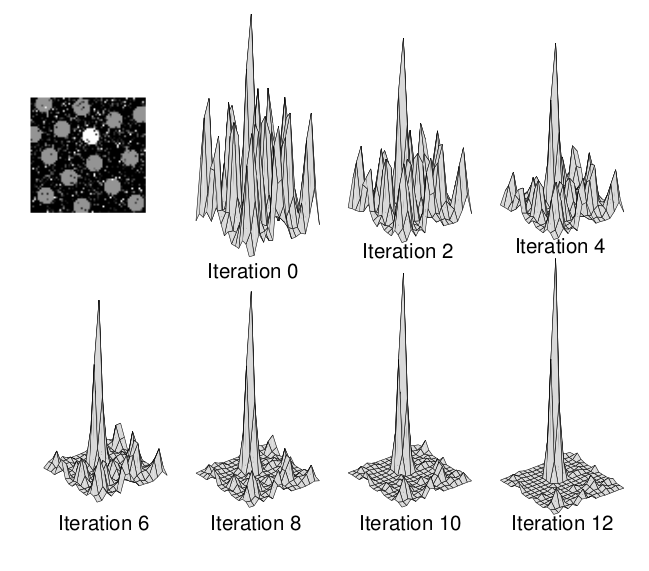
\includegraphics[width=3in]{迭代的局部交互.png}
\end{minipage}
\hspace{1ex}
\begin{minipage}[c]{1.0\textwidth}
\centering
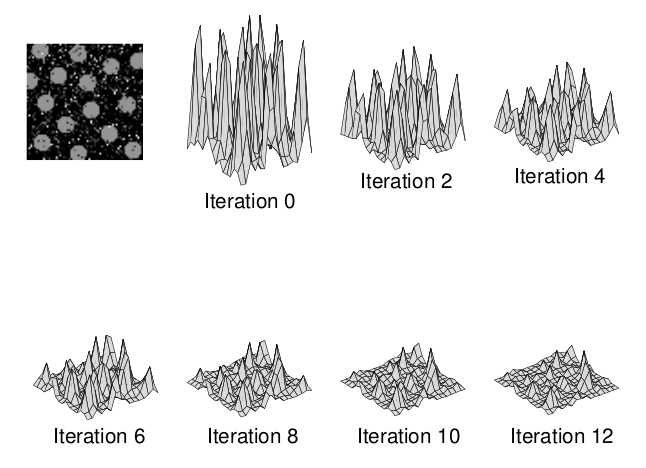
\includegraphics[width=3in]{迭代的局部交互2.png}
\end{minipage}
\caption{迭代的局部交互}\label{fig:10}
\end{figure} 

从图\ref{fig:10}中可以看出,6次迭代之后的效果就已经很明显了。Itti通过多次试验,认为将迭代次数设置为10比较合适。尽管效果较好,但是每一个特征显著图都要进行10次迭代,这种方法的计算量非常大。
%主要介绍基于内容的全局缩放方法(附上全局缩放的理论图)

\section{特征显著图融合}

一直并行处理的特征信息最终会在视觉皮层中整合起来综合分析,特征融合就是用于模拟这种生理功能,将42个特征显著图合并为1个显著图。


上一步的特征显著图的竞争是一种归一化算子,记作$N(\cdot)$。再定义一种求和运算,将两幅图像缩放至高斯金字塔尺度4的大小,再逐像素相加,记作$\oplus$。


首先计算特征的总体显著图。亮度特征有6幅显著图、颜色特征有12幅显著图、方向特征有24幅显著图,属于同一类特征的显著图都有相同的量纲和意义,经过归一化之后可以直接合并在一起。公式如下:
\begin{equation}
\bar{I}=\oplus_{c=2}^{4}\oplus_{s=c+3}^{c+4}N(I(c,s))
\end{equation}
\begin{equation}
\bar{C}=\oplus_{c=2}^{4}\oplus_{s=c+3}^{c+4}[N(RG(c,s))+N(BY(c,s))]
\end{equation}
对于方向特征,首先将每个方向的6幅显著图合并起来,得到4幅显著图,每个方向1幅。再把这4幅归一化之后合并起来,得到方向特征的总体显著图。

\begin{equation}
\bar{O}=\Sigma_{\theta\in\{0^\circ,45^\circ,90^\circ,135^\circ \}}N(\oplus_{c=2}^{4}\oplus_{s=c+3}^{c+4}N(O(\theta,c,s)))
\end{equation}

\begin{figure}[!ht]
\begin{minipage}[c]{0.31\textwidth}
\centering
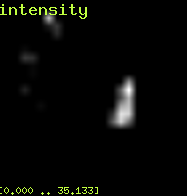
\includegraphics[width=1.25in]{intensity_map.png}
\end{minipage}
\hspace{1ex}
\begin{minipage}[c]{0.31\textwidth}
\centering
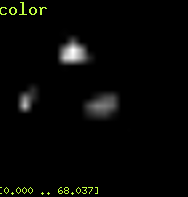
\includegraphics[width=1.25in]{color_map.png}
\end{minipage}
\hspace{1ex}
\begin{minipage}[c]{0.31\textwidth}
\centering
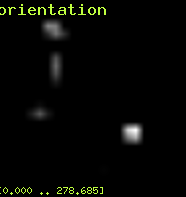
\includegraphics[width=1.25in]{orientation_map.png}
\end{minipage}
\caption{亮度、颜色、方向特征显著图}\label{fig:11}
\end{figure} 


得到特征的总体显著图后,需要对不同的特征进行合并。不同的特征具有不同的意义与量纲,比如5\%的亮度与$10^\circ$的方向哪个引起的视觉注意更强烈,是难以直接比较的。Itti模型对这个问题进行了简化,对不同特征的总体显著图归一化,从数量上保证它们的可比性,然后直接求取平均值:

\begin{equation}
S=\frac{1}{3}(N(\bar{I})+N(\bar{C})+N(\bar{O}))
\end{equation}

\begin{figure}[!htb]
\centering
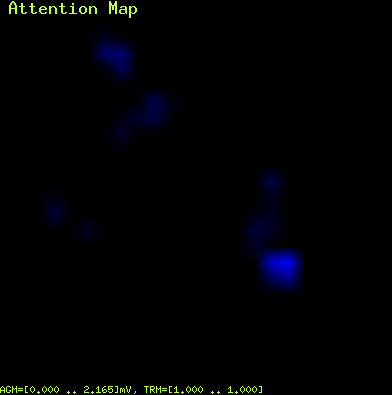
\includegraphics[width=0.3\textwidth]{map.png}
\caption{最终显著图}
\label{fig:12} 
\end{figure}




%利用归一化算子及求和求平均运算获得显著图(附上显著图)

\section{注意焦点转移}

心理实验表明,人眼的注意焦点是不断变化的,而且注意焦点的轨迹是环形的结构,即一个区域被注视之后,短时间内不会再被注意到,但过了一段时间以后又会引起视觉注意,注意焦点就在少数的感兴趣区域不断转移、循环。Itti 模型模拟了大脑皮层中的反馈抑制机制,实现了注意焦点转移的功能。


视觉系统会首先注意到当前显著图中最显著的区域,Itti模型利用一个“赢者通吃”(winner-take-all, WTA)的神经网络来实现这个功能。不但可以快速的找到显著值最大的区域,也更加具有生理意义。


然而仅依靠一个 WTA 神经网络,注意焦点将始终固定在图像中的一个位置。为了实现注意焦点的转移,Itti,模型从 WTA 网络中引出一个反馈信号来抑制显著图。当 WTA网络计算出一个最显著的位置时,将显著图中这个位置及其周围区域的显著值降低。这样再通过 WTA 网络计算出的显著位置就是之前的次显著位置,从而实现了注意焦点的转移。这种机制被称为返回抑制(inhibition of return)。实验结果如图\ref{fig:13}所示,利用法则来寻找显著区域的位置和尺寸,并将注意后的区域的显著度值设置为最小来抑制该区域再次被返回。

\begin{figure}[!ht]
\begin{minipage}[c]{0.22\textwidth}
\centering
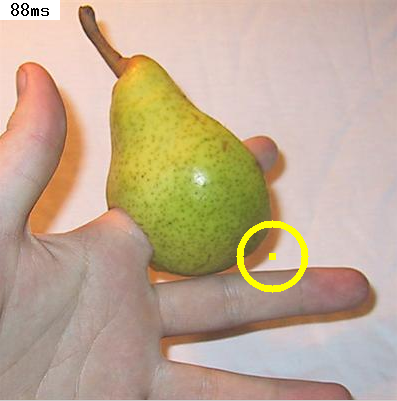
\includegraphics[width=1in]{视觉转移1.png}
\end{minipage}
\hspace{2ex}
\begin{minipage}[c]{0.22\textwidth}
\centering
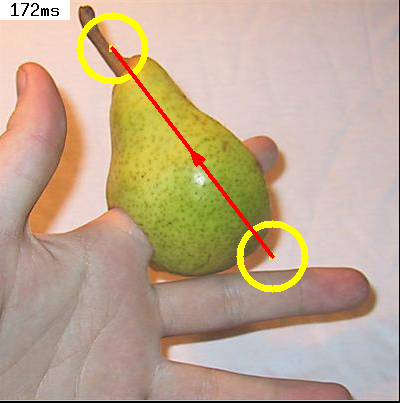
\includegraphics[width=1in]{视觉转移2.png}
\end{minipage}
\hspace{2ex}
\begin{minipage}[c]{0.22\textwidth}
\centering
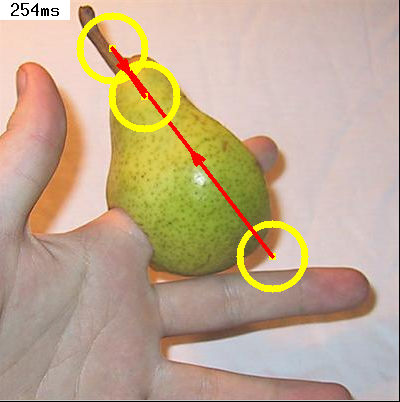
\includegraphics[width=1in]{视觉转移3.png}
\end{minipage}
\hspace{2ex}
\begin{minipage}[c]{0.22\textwidth}
\centering
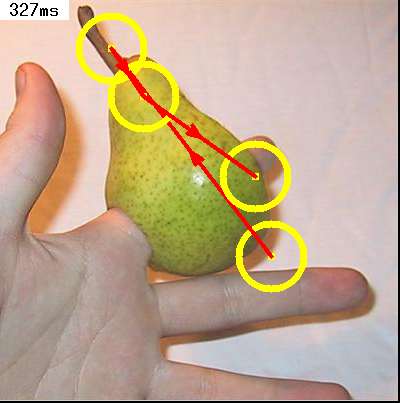
\includegraphics[width=1in]{视觉转移4.png}
\end{minipage}
\caption{视点转移过程}\label{fig:13}
\end{figure} 
%通过WTA机制及抑制返回机制最终获得注意焦点的转移(附上注意转移的图像)

\section{总结与展望}

详细介绍了Itti等人建立的视觉注意机制计算模型。该模型严格的模拟了人类系统,具有良好的生理依据。该模型首先提取亮度、颜色、方向等底层特征,然后通过DOG函数计算特征显著图,特征显著图又经过了竞争与融合,最终通过一个返回抑制网络实现注意点的选择与转移。从结果上看,该模型效果较好,因此得到了广泛的关注与应用。


尽管Itti视觉注意模型有上述优点,但在该模型中仍存在下面几点较为明显的问题。第一,由于模型中采用多尺度特征计算,以及在显著度计算中采用了较为复杂的一算子,故使得模型的整体计算量较大,违背了自底向上视觉注意过程中快速的特点第二,在多特征显著度图融合的过程中,模型中认为每个特征通道的贡献是均等的。但实际上,这样的假设并不合理。许多心理学研究工作表明,人眼在观察物体时,对于某些特征具有倾向性,并且特征之间是竞争与协作的关系。第三,由于多尺度特征图的融合,显著对象的边缘信息已经丢失,使得在最终的显著度图中只能通过一算子进行固定尺寸的圆形区域来模糊地描述视觉显著对象的大致位置,而无法准确地表达显著对象的外形轮廓,这对于许多图像分析任务是不够精确的。


通过对Itti视觉注意模型的整理,深切体会到Itti所做的工作为图像处理开辟了一个新天地,他将视觉生理功能适当简化并用计算模型表示出来,尽管存在一些缺点,但他的思想将给后人更多的启发。目前,在Itti模型的基础上改进的模型正一步步的发展起来,通过对Itti模型的学习,希望自己在今后能够对其模型进行不断完善。


由于人类视觉注意机制是一个复杂的系统,目前其工作机理尚不明确,因此作为一个涉及心理学、认知神经科学和计算机视觉等前沿领域的交叉学科,该学科还有许多问题仍待解决。本文仅仅针对Itti视觉注意模型进行的整理,其研究的深度与广度都具有一定的局限性。今后还要继续关注各交叉学科的动态发展,更深刻的来理解视觉注意建模的理论和思想,为下一步视觉注意模型的改进工作打下基础。


%回顾本文的内容,提出自己的感受,介绍今后的工作。


\bibliographystyle{plain}
\bibliography{IttiModel}


\end{document}
